\documentclass{article}
\usepackage{fullpage}
\usepackage{graphicx} % Required for inserting images
\usepackage{xcolor, xspace}
\usepackage{hyperref}
\usepackage{subcaption}


\newcommand{\todo}[1]{\xspace\textcolor{red}{[\ TODO:\ #1\ ]}\xspace}

\title{RAG for CS\&Law}
\author{Julie Ha}
\date{May 2026}

\begin{document}

\maketitle
\section{Introduction}
There is an emerging field of research at the intersection of computer science and law, which explore how computational techniques can be applied to legal problems, and how the rise of technology impacts and raises new questions in the legal domain. 
This field, aptly named CS\&Law, results in collaborations between experts in both domains. 
These collaborations require both parties to learn about the other's field, while also looking through previous related literature. 
Searching for literature in a unfamiliar field could be a challenge for researchers who lack domain-specific expertise. 
Motivated by this problem, I created a RAG pipeline, specifically made for CS\&Law papers. 

\section{Approach}
I followed a classic RAG approach, finding documents, chunking, embedding, and then asking questions. 
\subsection{Finding Documents}
The corpus was built from publications from ACM CS\&Law~\cite{cslaw_2026}.
Because only four years of formal publications were available,\footnote{Although the website includes a tab for 2019, that year did not contain formal publications and appeared to be organized more like a workshop.} the proceedings for each year were reviewed and the corresponding PDFs were downloaded. 

\subsection{Finding Citations}
Since this RAG pipeline's main purpose is to be a research tool, it would be helpful for the RAG to return citations alongside its answers, so a user would be able to find and read the full text of the relevant paper. 
While classic RAG implementations will show retrieved chunks, there was not a standard way to return citations alongside the chunks. 
To make this an effective tool, the RAG query needed to retrieve the citation for the paper. 
To implement this, an agent was developed to look up each citation based on the PDF file name. 
Because the file names were partially formatted as DOIs, they could be converted into searchable DOI strings more easily. 
In the event that searching for the DOI failed, the first 500 characters of the first page were utilized by the agent to find the paper.
After the citations were successfully found, the IEEE citation was added to the metadata of the PDF, which would also be added to each of the chunks in the chunking step. 

\subsection{Chunking Documents}
Fixed size chunking, document structure aware chunking, sentence based chunking, and semantic chunking were all implemented to compare retrieval. 
Semantic chunking relied on the package \texttt{SemanticChunker} from \texttt{langchain\_experimental}. 

\subsection{Embedding Model}
One of the goals I wanted from this project was to make everything accessible, which meant everything had to basically been using a free-tier AI model. 
Thus, for the embedding model, a free tier API from HuggingFace was used, specifically \texttt{sentence-transformers/all-MiniLM-L6-v2}. 
I had started with building a RAG pipeline that only had fixed sentence chunking, and later added the other methods. 
As a result, my most recent iteration of my code has an embedding model that is best suited for a fixed size chunking or sentence-based chunking approach, but applied on all four methods. 
\paragraph{Future Work} With more time, I would probably try to find embedding models that are better suited for each of the different methods. 

\subsection{Retrieval}
Retrieval by vector similarity search, MMR, scores, threshold, BM25, and hybrid retrieval were implemented to compare retrieval methods. 

\subsection{Answer Generation}
To focus on using free tier AI models, TinyLlama-1.1B-Chat-v1.0 was used for RAG answer generation. 

\section{Results and Discussion}

\subsection{Precision and Recall}
Precision and recall were tested with set of questions that had expected answers. 
This set was generated with assistance from Codex, as well as the evaluation code. 
Precision and recall were tested against the different chunking methods, and the different retrieval methods. 
\begin{figure}[ht]
    \centering

    \begin{subfigure}{0.48\textwidth}
        \centering
        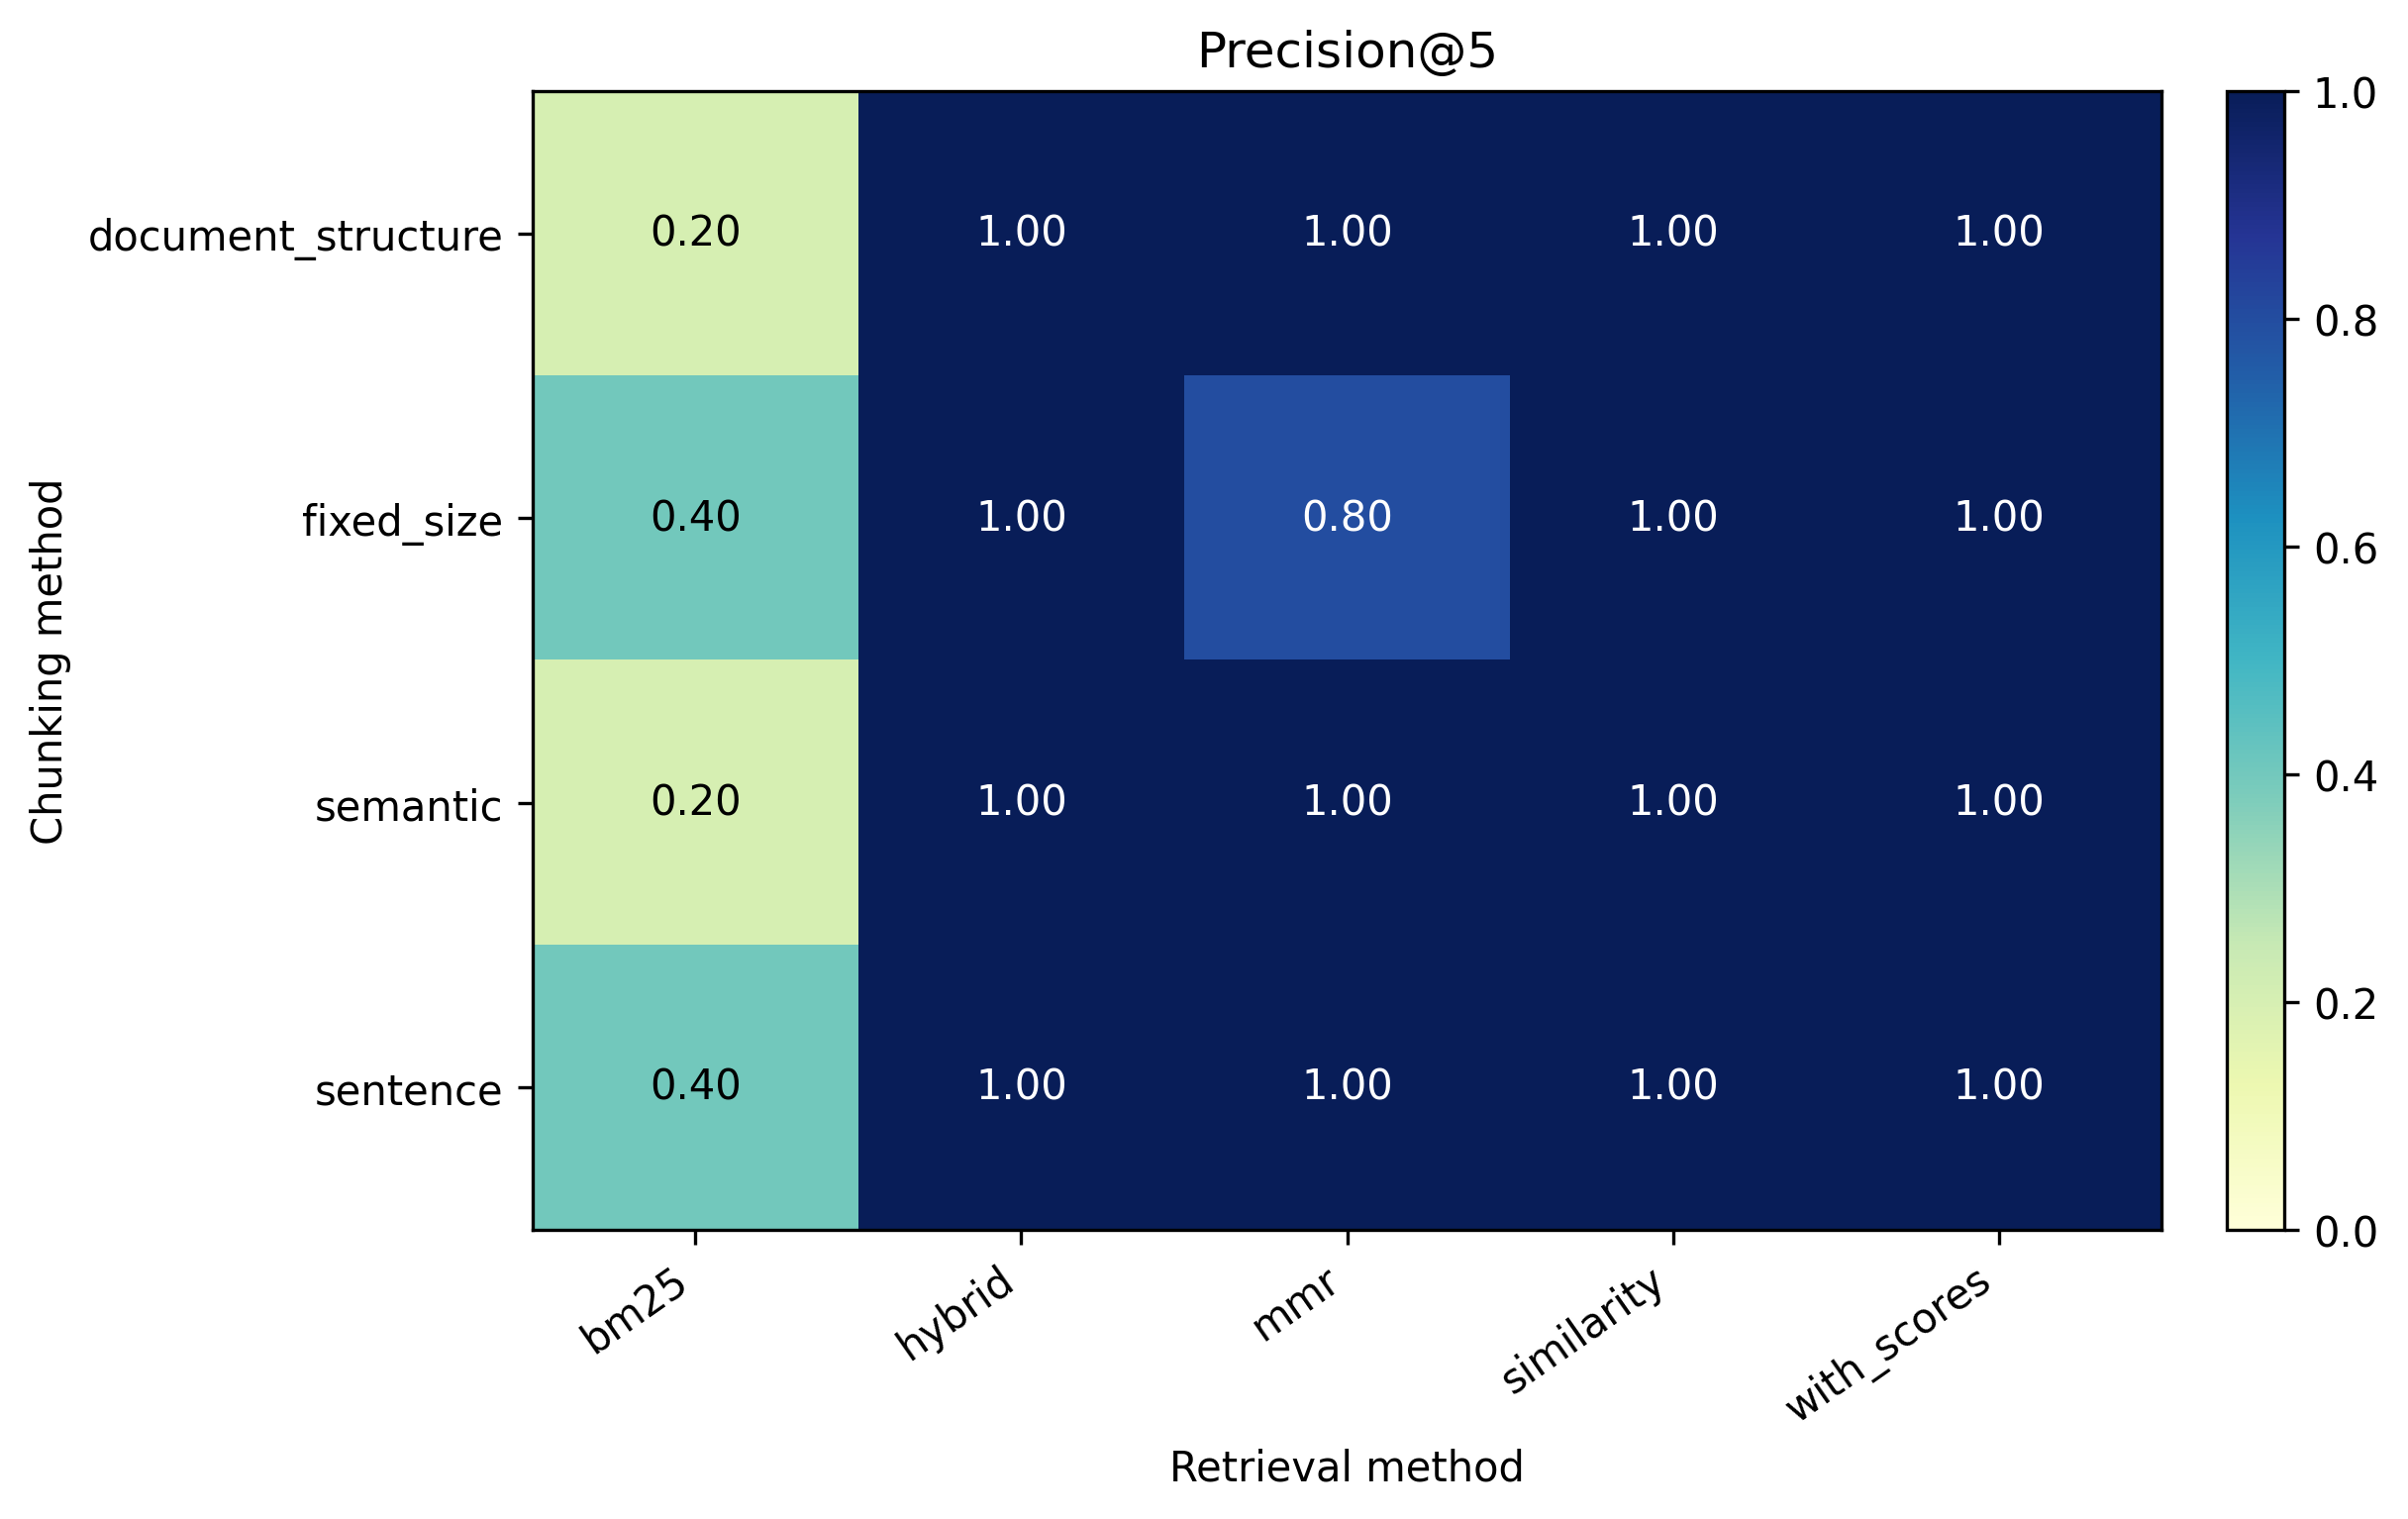
\includegraphics[width=\textwidth]{attachments/precision_heatmap_k5.png}
        \caption{Heat map for precision}
        \label{fig:precision}
    \end{subfigure}
    \hfill
    \begin{subfigure}{0.48\textwidth}
        \centering
        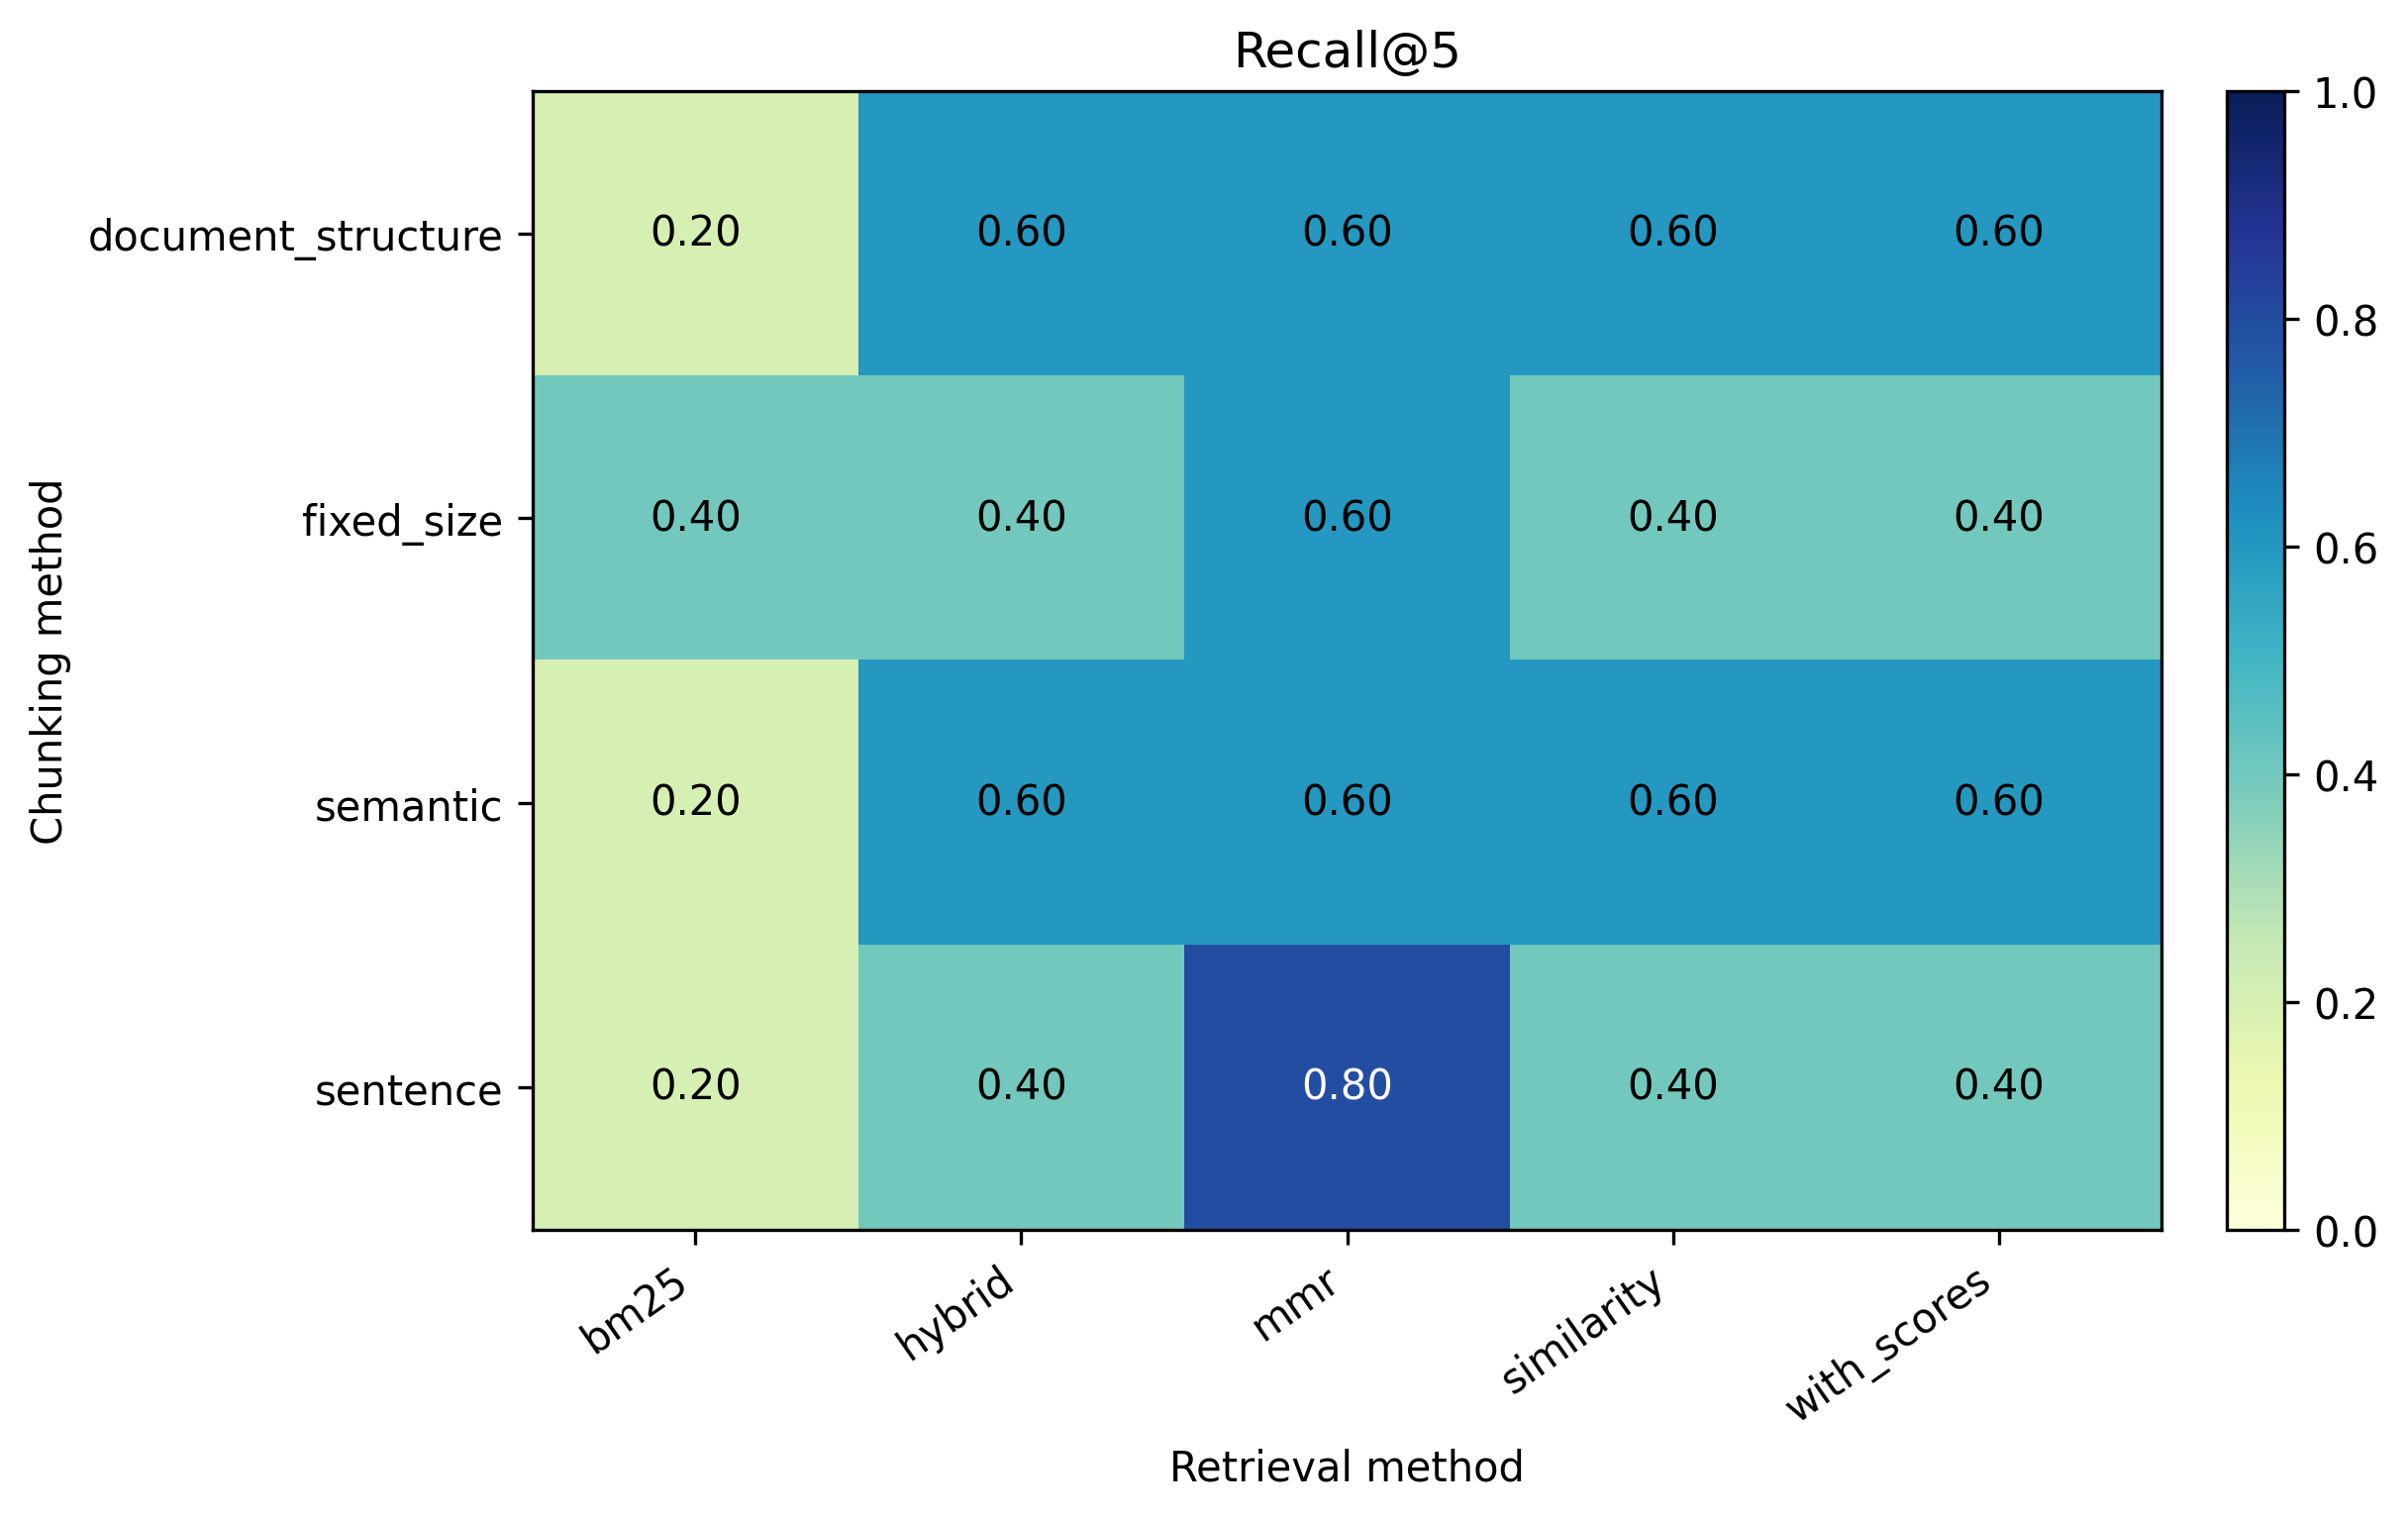
\includegraphics[width=\textwidth]{attachments/recall_heatmap_k5.png}
        \caption{Heat map for recall}
        \label{fig:recall}
    \end{subfigure}

    \label{fig:precision-recall}
\end{figure}

For precision and recall, BM25 did signficantly worse than the other methods. 
Otherwise, precision was similar across different chunking and retrieval methods. 
For recall, MMR with sentence level chunking had the best recall, while semantic and document-structure chunking fell slightly behind. 

\paragraph{Limitation} It is relevant to note that the test set was quite small. 
With more time, a bigger test set would yield more accurate results. 

\subsection{Obstacles and Unsuccessful Attempts}
\paragraph{Google Colab}
The project was initially developed in Google Colab, which had been a useful tool throughout the semester and helped avoid package installation issues or compatibility problems on a local machine. 
However, working in Colab introduced significant limitations, including slower computation and the inability to use Ollama.
As a result, the project was moved to a local implementation, which allowed for different package installs and faster computation. 
\paragraph{Slow Vector DB Creation}
While not necessarily an obstacle, creating the vector DB in Google Colab took considerably long, taking around 12 minutes. 
Once the project was moved over to a local machine, creating the vector DB was considerably faster, taking around 30 seconds, regardless of the chunking method used. 
\paragraph{Choice of LLM Model}
To make the implementation more accessible, a free-tier AI model was preferred, making Ollama~\cite{ollama_llama31} a strong candidate.
Llama 3.1 is an openly available model from Meta, and has different models with different numbers of parameters. 
An initial attempt was made to run \texttt{ollama3.1:8b}, which produced the following error:
\begin{center}
    \texttt{Error: 500 Internal Server Error: llama runner process has terminated: \%!w(<nil>)}
\end{center}
Although the model was loaded on the local machine, the error was initially assumed to be caused by the model size. 
To test this, smaller models were attempted, including \texttt{ollama3.2:3b} and \texttt{qwen2.5:0.5b}, with Qwen2.5 having significantly fewer parameters than the other Ollama models. 
However, both produced the same error.

The issue was later found to be a compatibility problem: the newest version of Ollama was not yet compatible with the Apple M5 chip~\cite{ollama_issue_15448}. 
Although downgrading Ollama to version 0.20.3 may have been possible, Ollama was ultimately removed from the implementation in favor of \texttt{TinyLlama-1.1B-Chat-v1.0} from HuggingFace, which had worked reliably in previous use.

\section{Ethics and Limitations}
Because the tool was primarily developed for personal use, it presents limited ethical concerns. 
Even if deployed more broadly, its intended purpose is to support literature discovery and knowledge exploration, which suggests minimal ethical impact.
However, since the corpus is made of papers from strictly CS\&Law, it is not a comprehensive literature search tool, as it is missing works from law journals that discuss tech topics. 

\section{Future Work}
\subsection{Further Publications}
The corpus can be expanded to legal journals, which sometimes have articles that are either written by computer scientists or are about the impact of tech in the legal domain. 
One can imagine that there will be a bit more difficulty with filtering out this corpus; while there are law journals specific to tech such as~\cite{yale_jolt}. 
However, expanding the corpus to legal journals will allow for further perspective on this field. 
Additionally, law journals are often a resource that are used for researchers doing work in the field, so integrating law journals will make the RAG pipeline more useful. 

\subsection{Crypto.bib}
For this project, a set of documents was downloaded, and an agent was created to find the IEEE citations of the documents in the corpus. 
This project also suggests a different application using Crypto.bib~\cite{cryptobib}: a large, continually updated BibTeX file containing citations for cryptography-related publications. 
Cryptographers often use this file to cite relevant papers, since it avoids the need to manually create a separate BibTeX file for each LaTeX project.

Crypto.bib could also serve as a useful foundation for a RAG pipeline. 
Rather than starting with downloaded PDFs and then identifying citations, the citation database could be used to locate PDFs directly and update the RAG corpus as new citations are added. 
This system could be a helpful resource for junior researchers by supporting literature searches, identifying related work, and recommending papers to read.

\subsection{Compare different models}
With more time, future work could compare the performance of different AI models for answer generation. 
This could include configuring an earlier compatible version of Ollama locally and comparing its outputs against those produced by \texttt{TinyLlama-1.1B-Chat-v1.0}. 

\subsection{Human Evaluation}
A rigorous human evaluation of the generated answers was not completed due to time constraints. 
Future work could involve reviewing the generated answers saved in the GitHub repository and scoring them on a 0-1-2 scale, where 0 indicates an irrelevant answer, 1 indicates a partially relevant answer, and 2 indicates a high-quality answer.

\nocite{*}
\bibliographystyle{alpha}
\bibliography{refs}
\end{document}
